% Présentation Lifen, partie 1 : une heuristique pour retrouver le nom du patient
% Compilation : tectonic presentation_heuristique.tex
% Les figures (dossier figures/) viennent des vraies boîtes JSON et du code de l'heuristique.
\documentclass[11pt,aspectratio=169]{beamer}

\usefonttheme{serif}
\usefonttheme{professionalfonts}
\usepackage{amsmath,amssymb}
\usepackage{fontspec}            % Latin Modern, la police par défaut de LaTeX
\usepackage[english,french]{babel}
\usepackage{booktabs}
\usepackage{array}
\usepackage{listings}
\usepackage[noend]{algpseudocode}
\usepackage{tikz}
\usetikzlibrary{arrows.meta,positioning,calc,babel}
\usepackage{pgfplots}            % courbes ROC et précision–rappel (§ 4.7, 4.8)
\pgfplotsset{compat=1.17}
\graphicspath{{figures/}}

% Couleurs des figures : palette par défaut de matplotlib
\definecolor{mlblue}{HTML}{1F77B4}
\definecolor{mlorange}{HTML}{FF7F0E}
\definecolor{mlgreen}{HTML}{2CA02C}
\definecolor{mlred}{HTML}{D62728}
\definecolor{mlpurple}{HTML}{9467BD}
\definecolor{mlgray}{HTML}{7F7F7F}
% Les mêmes, un peu plus sombres pour le texte
\colorlet{tblue}{mlblue!85!black}
\colorlet{torange}{mlorange!80!black}
\colorlet{tgreen}{mlgreen!75!black}
\colorlet{tred}{mlred!90!black}
\colorlet{tpurple}{mlpurple!85!black}

% Mise en page sobre, comme un article : texte noir, titres en gras
\setbeamercolor{normal text}{fg=black,bg=white}
\setbeamercolor{structure}{fg=black}
\setbeamerfont{title}{series=\bfseries,size=\LARGE}
\setbeamerfont{subtitle}{series=\mdseries,shape=\itshape,size=\normalsize}
\setbeamerfont{frametitle}{series=\bfseries,size=\large}
\setbeamerfont{caption}{size=\scriptsize}
\setbeamertemplate{navigation symbols}{}
\setbeamertemplate{itemize item}{\textbullet}
\setbeamertemplate{enumerate item}{\insertenumlabel.}
\setbeamertemplate{footline}{%
  \leavevmode
  \hbox to \paperwidth{\hskip1cm\color{mlgray}\scriptsize
    Retrouver le nom du patient\hfill\insertframenumber\,/\,\inserttotalframenumber\hskip1cm}%
  \vskip2.5mm}

\newcommand{\pct}[1]{#1\,\%}
\newcommand{\en}[1]{\foreignlanguage{english}{#1}}
% Un mot exact du document ou du code, sans l'espace que le français ajoute avant « : »
\newcommand{\tok}[1]{\foreignlanguage{english}{\texttt{#1}}}
\newcolumntype{L}[1]{>{\raggedright\arraybackslash}p{#1}}
% Mots colorés comme dans les figures
\newcommand{\civ}[1]{\textcolor{torange}{\bfseries #1}}   % civilité
\newcommand{\nm}[1]{\textcolor{tgreen}{\bfseries #1}}     % nom lu
\newcommand{\drt}[1]{\textcolor{tred}{\bfseries #1}}      % titre de médecin
\newcommand{\lab}[1]{\textcolor{tpurple}{\bfseries #1}}   % étiquette de formulaire
\newcommand{\ctx}[1]{\textcolor{mlgray}{#1}}              % mot de contexte
\newcommand{\figcap}[1]{{\color{mlgray}\scriptsize #1}}  % légende de figure

% Courbes ROC et précision–rappel : mêmes axes et mêmes marques que dans la partie 2
\pgfplotsset{
  courbe/.style={
    width=5.3cm, height=5.3cm,
    xmin=0, xmax=1, ymin=0, ymax=1.02,
    xtick={0,0.5,1}, ytick={0,0.5,1},
    /pgf/number format/use comma,
    tick label style={font=\scriptsize},
    label style={font=\scriptsize},
    axis line style={black!60}, tick style={black!60},
    legend style={font=\scriptsize, draw=none, fill=white, row sep=-1pt},
    legend cell align=left,
    clip=false},
  minimale/.style={mlgray, thick, mark=*, mark size=1.5pt},
  miseenpage/.style={mlblue, thick, mark=square*, mark size=1.4pt},
  seuilactuel/.style={only marks, mark=o, mark size=3.2pt, mlorange, very thick},
}
\tikzset{seuil/.style={font=\tiny, text=black!75, inner sep=1.5pt}}

% Code Python, comme dans un article
\lstset{
  language=Python,
  basicstyle=\ttfamily\fontsize{7}{8}\selectfont,
  keywordstyle=\bfseries,
  morekeywords={None},
  showstringspaces=false,
  columns=fullflexible,
  keepspaces=true,
  upquote=true,
  aboveskip=0pt,
  belowskip=0pt,
  literate={é}{{\'e}}1
}

% Algorithmes, comme dans un article : mots-clés en français, encadré par des filets
\algrenewcommand\algorithmicrequire{\textbf{Entrée :}}
\algrenewcommand\algorithmicensure{\textbf{Sortie :}}
\algrenewcommand\algorithmicfor{\textbf{pour}}
\algrenewcommand\algorithmicforall{\textbf{pour chaque}}
\algrenewcommand\algorithmicdo{\textbf{faire}}
\algrenewcommand\algorithmicif{\textbf{si}}
\algrenewcommand\algorithmicthen{\textbf{alors}}
\algrenewcommand\algorithmicelse{\textbf{sinon}}
\algrenewcommand\algorithmicreturn{\textbf{retourner}}
\algnewcommand\algorithmicforeach{\textbf{pour chaque}}
\algdef{S}[FOR]{ForEach}[1]{\algorithmicforeach\ #1\ \algorithmicdo}
\algrenewcommand{\algorithmiccomment}[1]{\hfill{\color{mlgray}$\triangleright$ #1}}
\algrenewcommand\alglinenumber[1]{{\scriptsize\color{mlgray}#1}}
\newenvironment{algo}[1]{%
  \par\noindent\rule{\linewidth}{0.8pt}\par\vspace{2pt}%
  \noindent\footnotesize #1\par\vspace{-4pt}%
  \noindent\rule{\linewidth}{0.4pt}\par\vspace{-2pt}%
}{%
  \par\vspace{-6pt}\noindent\rule{\linewidth}{0.8pt}\par
}

\title{Retrouver le nom du patient}
\subtitle{Une heuristique à base de règles : où elle échoue,\\ et comment la mise en page la corrige}
\author{Alexandre Rogojan}
\institute{Lifen \,·\, stage Machine Learning Engineer \,·\, partie 1}
\date{}

\begin{document}

\begin{frame}[plain]
  \titlepage
\end{frame}

% ---------------------------------------------------------------------------
\begin{frame}{1\quad La tâche : un JSON en entrée, un nom en sortie}
  \begin{columns}[T]
    \column{0.30\textwidth}
    \textbf{Entrée}\par\smallskip
    \small Chaque mot de la page avec sa boîte : $x$ et $y$ vont de 0 à 1 depuis le
    coin en haut à gauche. Les mots arrivent dans un ordre quelconque.
    \column{0.30\textwidth}
    \textbf{Sortie}\par\smallskip
    \small Le prénom et le nom du patient, ou \tok{None} quand le document ne donne aucun
    indice clair.
    \column{0.30\textwidth}
    \textbf{Contrainte}\par\smallskip
    \small L'heuristique la plus simple : pas d'apprentissage automatique, un code court que
    tout le monde peut lire.
  \end{columns}

  \vspace{1.4em}
  \textbf{Notation.} Une page est un ensemble de mots $D = \{(t_i, b_i)\}_{i=1}^{n}$, où
  $t_i$ est le texte du mot et $b_i = (x_i^{\min}, x_i^{\max}, y_i^{\min}, y_i^{\max}) \in [0,1]^4$
  sa boîte. On veut :
  \[
    f(D) = (\text{prénom}, \text{nom})
  \]
  \begin{center}
    \tok{find\_patient(document)} \;$\longrightarrow$\; \tok{('Jean', 'DUPONT')}
  \end{center}
\end{frame}

% ---------------------------------------------------------------------------
\begin{frame}[fragile]{1.1\quad Ce que contient le JSON}
  \begin{columns}[T]
    \column{0.30\textwidth}
    \centering
    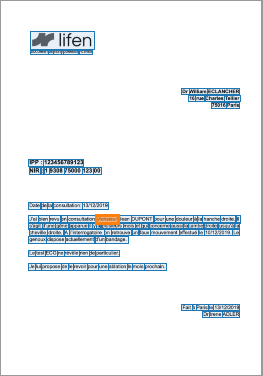
\includegraphics[height=5.6cm]{fig_json}\par\smallskip
    \figcap{Document 3 : une boîte par mot, «~Monsieur~» en orange.}
    \column{0.64\textwidth}
    \small Chaque mot est un objet JSON :

    \smallskip
    \begin{otherlanguage}{english}
\begin{lstlisting}[language={}]
{"text": "Monsieur",
 "bbox": {"x_min": 0.37, "x_max": 0.45,
          "y_min": 0.57, "y_max": 0.59}}
\end{lstlisting}
    \end{otherlanguage}

    \medskip
    Un extrait de la page, dans un ordre quelconque :

    \smallskip
    {\footnotesize
    \begin{tabular}{@{}lcccc@{}}
      \toprule
      \tok{text} & \tok{x\_min} & \tok{x\_max} & \tok{y\_min} & \tok{y\_max} \\
      \midrule
      \tok{jusqu'à} & \tok{0.83} & \tok{0.89} & \tok{0.59} & \tok{0.61} \\
      \tok{douleur} & \tok{0.67} & \tok{0.74} & \tok{0.57} & \tok{0.59} \\
      \textcolor{torange}{\tok{Monsieur}} & \textcolor{torange}{\tok{0.37}} & \textcolor{torange}{\tok{0.45}}
        & \textcolor{torange}{\tok{0.57}} & \textcolor{torange}{\tok{0.59}} \\
      \tok{123} & \tok{0.31} & \tok{0.35} & \tok{0.45} & \tok{0.46} \\
      \tok{s'agit} & \tok{0.11} & \tok{0.16} & \tok{0.59} & \tok{0.61} \\
      \bottomrule
    \end{tabular}}

    \medskip
    \begin{itemize}
      \item 110 mots lus par OCR. $x$ : 0 au bord gauche, 1 au bord droit ; $y$ : 0 en
        haut, 1 en bas.
      \item Seules les boîtes disent où est un mot : l'heuristique ne lit jamais l'image.
    \end{itemize}
  \end{columns}
\end{frame}

% ---------------------------------------------------------------------------
\begin{frame}{2\quad L'heuristique minimale : deux règles, dans l'ordre}
  \begin{columns}[T]
    \column{0.86\textwidth}
    \begin{algo}{\textbf{Algorithme 1 :} heuristique minimale (\tok{find\_patient})}
    \begin{algorithmic}[1]
      \Require un document : des pages, chacune avec ses mots et leurs boîtes
      \Ensure (prénom, nom) du patient, ou \tok{None}
      \ForEach{page du document}
        \State $m_1, \dots, m_k \gets$ les mots de la page dans l'ordre de lecture
          \Comment{étape 1}
        \If{un mot $m_i$ vaut \tok{Nom:}} \Comment{règle 1}
          \State \Return (mot après \tok{Prénom:}, mot après \tok{Nom:})
        \EndIf
        \ForEach{civilité $m_i$ (Monsieur, Madame, Mme…)} \Comment{règle 2}
          \If{$m_{i-1}$ n'est pas un titre de médecin (Dr, Docteur, Pr…)}
            \State $N \gets$ au plus deux mots après $m_i$, arrêt au premier mot en minuscule
            \State \textbf{si} $N = (n)$, \Return (\tok{None}, $n$) ;
              \textbf{si} $N = (p, n)$, \Return $(p, n)$
          \EndIf
        \EndFor
      \EndFor
      \State \Return \tok{None}
    \end{algorithmic}
    \end{algo}
  \end{columns}

  \vspace{0.8em}
  \begin{center}
    \small La première règle qui trouve un nom répond : aucun score, aucune comparaison.
  \end{center}
\end{frame}

% ---------------------------------------------------------------------------
\begin{frame}[fragile]{2.1\quad Étape 1 : remettre les mots dans l'ordre de lecture}
  \lstset{basicstyle=\ttfamily\fontsize{6.4}{7.6}\selectfont}
  \begin{columns}[T]
    \column{0.49\textwidth}
    \small
    \begin{enumerate}
      \item Trier les mots par $(y^{\min}, x^{\min})$.
      \item Nouvelle ligne quand $y^{\min}$ saute de plus de $\delta = 0{,}005$.
      \item Trier chaque ligne par $x^{\min}$.
    \end{enumerate}

    \medskip
    \textbf{Pourquoi des lignes ?} Sur le document 1, «~Juliette~» est $0{,}0003$ plus
    bas que ses voisins :

    \smallskip
    \begin{center}
      \begin{tikzpicture}[w/.style={draw=black!60, font=\footnotesize, inner sep=2.5pt,
                                    minimum height=0.45cm, anchor=south west}]
        \node[w] (a) at (0, 0) {Madame};
        \node[w] (b) at ($(a.south east) + (0.06, -0.14)$) {Juliette};
        \node[w] (c) at ($(b.south east) + (0.06, 0.14)$) {MARTIN};
        \foreach \n/\y in {a/0.1017, b/0.1020, c/0.1017}
          \node[below=0pt of \n, font=\tiny, text=mlgray] {\tok{\y}};
      \end{tikzpicture}
    \end{center}

    \footnotesize
    \begin{tabular}{@{}ll@{}}
      $(y, x)$ seul : & \tok{Madame MARTIN Juliette} \textcolor{tred}{$\times$} \\
      lignes, puis $x$ : & \tok{Madame Juliette MARTIN} \textcolor{tgreen}{\checkmark}
    \end{tabular}

    \column{0.48\textwidth}
    \begin{otherlanguage}{english}
\begin{lstlisting}
def read_words(page):
    words = []
    for word in page["words"]:
        y = word["bbox"]["y_min"]
        x = word["bbox"]["x_min"]
        words.append((y, x, word["text"]))
    words.sort()
    lines = []
    previous_y = 0
    for y, x, text in words:
        if len(lines) == 0 or y - previous_y > LINE_GAP:
            lines.append([])
        lines[-1].append((x, text))
        previous_y = y
    result = []
    for line in lines:
        line.sort()
        for x, text in line:
            result.append(text)
    return result
\end{lstlisting}
    \end{otherlanguage}
  \end{columns}
\end{frame}

% ---------------------------------------------------------------------------
\begin{frame}{2.2\quad Règle 1 : un formulaire, \tok{Nom:} et \tok{Prénom:}}
  \begin{center}
    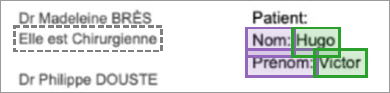
\includegraphics[width=0.62\textwidth]{fig_rule1}\par
    \figcap{Document 2 : les étiquettes en violet, les mots qui les suivent en vert.}
  \end{center}

  \small
  Dans l'ordre de lecture : \ctx{\tok{… BRÊS Patient: Elle est Chirurgienne}}
  \lab{\tok{Nom:}} \nm{\tok{Hugo}} \lab{\tok{Prénom:}} \nm{\tok{Victor}} \ctx{\tok{…}}

  \medskip
  \begin{itemize}
    \item On garde le mot qui suit \tok{Nom:} et celui qui suit \tok{Prénom:}, ce qui
      donne \tok{('Victor', 'Hugo')}.
    \item La ligne mélange les deux colonnes («~Elle est Chirurgienne~» vient de la colonne
      de gauche), mais le mot juste après \tok{Nom:} reste «~Hugo~».
    \item La comparaison est exacte : \tok{Nom :} (avec une espace) ou
      \tok{Nom de naissance :} ne déclenchent pas la règle. Pas de \tok{Nom:} sur la page :
      la règle 2 prend le relais.
  \end{itemize}
\end{frame}

% ---------------------------------------------------------------------------
\begin{frame}{2.3\quad Règle 2 : la première civilité qui ne suit pas un titre de médecin}
  Puis lire au plus deux mots après elle, tant qu'ils commencent par une majuscule.

  \vspace{0.8em}
  \begin{center}
    \small
    \renewcommand{\arraystretch}{1.25}
    \begin{tabular}{@{}L{2.0cm}L{5.4cm}L{5.4cm}@{}}
      \toprule
      \textbf{Document} & \textbf{Mots, dans l'ordre de lecture} & \textbf{Résultat} \\
      \midrule
      Document 3 & \ctx{consultation} \civ{Monsieur} \nm{Jean} \nm{DUPONT} \ctx{pour}
        & \tok{('Jean', 'DUPONT')} \\
      Document 1 & \ctx{Timone} \civ{Madame} \nm{Juliette} \nm{MARTIN}
        & \tok{('Juliette', 'MARTIN')} \\
      Document 1, plus bas & \ctx{le} \drt{docteur} \civ{Monsieur} Nicolas JACQUES
        & ignoré : le mot d'avant est un titre de médecin \\
      Document 2 & \ctx{revoir} \civ{Mme} \nm{HUGO} \ctx{\itshape un} \ctx{jour}
        & \tok{(None, 'HUGO')} : «~un~» est en minuscule \\
      \bottomrule
    \end{tabular}
  \end{center}

  \vspace{0.6em}
  \footnotesize
  \civ{Orange} : la civilité ; \nm{vert} : le nom lu ; \drt{rouge} : un titre de médecin juste
  avant. Sur le document 1, «~Madame~» répond avant que «~docteur Monsieur~» soit atteint ;
  sur le document 2, la règle 1 a déjà répondu.
\end{frame}

% ---------------------------------------------------------------------------
\begin{frame}[fragile]{2.4\quad Le code : des boucles et des \tok{if}, rien de plus}
  \lstset{basicstyle=\ttfamily\fontsize{6.6}{7.7}\selectfont}
  \begin{columns}[T]
    \column{0.36\textwidth}
    \textbf{Règle 1}\par\smallskip
    \begin{otherlanguage}{english}
\begin{lstlisting}
def find_patient(document):
    for page in document["pages"]:
        words = read_words(page)
        first_name = None
        last_name = None
        for i in range(len(words) - 1):
            word = words[i].lower()
            if word == "nom:":
                last_name = words[i + 1]
            if word == "prénom:":
                first_name = words[i + 1]
        if last_name is not None:
            return first_name, last_name
\end{lstlisting}
    \end{otherlanguage}
    \column{0.62\textwidth}
    \textbf{Règle 2}\par\smallskip
    \begin{otherlanguage}{english}
\begin{lstlisting}
        for i in range(len(words)):
            word = words[i].lower()
            if word not in CIVILITIES:
                continue
            if i > 0 and words[i - 1].lower() in DOCTOR_TITLES:
                continue
            name = []
            for j in range(i + 1, i + 3):
                if j >= len(words):
                    break
                if words[j].lower() in DOCTOR_TITLES:
                    break
                if not words[j][0].isupper():
                    break
                name.append(words[j].strip(".,"))
            if len(name) == 1:
                return None, name[0]
            if len(name) == 2:
                return name[0], name[1]
    return None
\end{lstlisting}
    \end{otherlanguage}
  \end{columns}

  \vspace{0.5em}
  \footnotesize
  62 lignes de code en tout, sans les commentaires : trois constantes, \tok{read\_words}
  et \tok{find\_patient}.
\end{frame}

% ---------------------------------------------------------------------------
\begin{frame}{2.5\quad Résultats sur les trois documents du challenge}
  \begin{columns}[T]
    \column{0.31\textwidth}
    \centering
    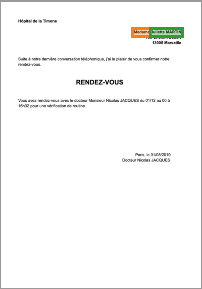
\includegraphics[height=4.6cm]{fig_doc1}\par\smallskip
    {\footnotesize (a) Règle 2, «~Madame~»\\ \tok{('Juliette', 'MARTIN')}}
    \column{0.31\textwidth}
    \centering
    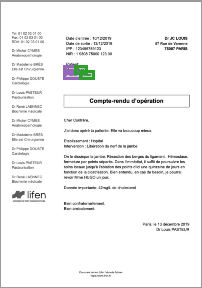
\includegraphics[height=4.6cm]{fig_doc2}\par\smallskip
    {\footnotesize (b) Règle 1, \tok{Nom:} et \tok{Prénom:}\\ \tok{('Victor', 'Hugo')}}
    \column{0.31\textwidth}
    \centering
    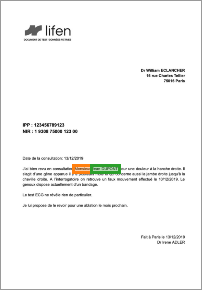
\includegraphics[height=4.6cm]{fig_doc3}\par\smallskip
    {\footnotesize (c) Règle 2, «~Monsieur~»\\ \tok{('Jean', 'DUPONT')}}
  \end{columns}

  \vspace{0.7em}
  \footnotesize
  En orange ou violet, l'indice ; en vert, le nom renvoyé. Aussi vérifié : 18 tests
  unitaires, les vraies boîtes OCR des trois pages, des mots mélangés et des lignes
  légèrement irrégulières.
\end{frame}

% ---------------------------------------------------------------------------
\begin{frame}{3\quad Où elle échoue : quatre documents ordinaires}
  \begin{center}
    \small
    \renewcommand{\arraystretch}{1.25}
    \begin{tabular}{@{}lllL{3.3cm}@{}}
      \toprule
      \textbf{Cas} & \textbf{Patient} & \textbf{Version minimale} & \textbf{Type d'erreur} \\
      \midrule
      Bandeau du personnel & Paul MOREAU & \textcolor{tred}{Sophie DURAND} & mauvaise personne \\
      Étiquette d'hôpital & Jean DUPONT & \tok{None} & aucune réponse \\
      Bloc d'identité & Camille LEROY & \tok{None} & aucune réponse \\
      Proche cité en premier & Pierre DURAND & \textcolor{tred}{Claire PETIT} & mauvaise personne \\
      \bottomrule
    \end{tabular}
  \end{center}

  \vspace{0.6em}
  \begin{itemize}
    \item \textbf{Mauvaise personne} : un faux positif, et le vrai patient est manqué. C'est
      l'erreur la plus grave : le document irait dans le dossier d'un autre patient.
    \item \textbf{Aucune réponse} : un faux négatif. Le document part en vérification
      humaine : coûteux, mais sans danger.
  \end{itemize}
\end{frame}

% ---------------------------------------------------------------------------
\begin{frame}{3.1\quad Elle renvoie la mauvaise personne}
  \begin{columns}[T]
    \column{0.48\textwidth}
    \centering
    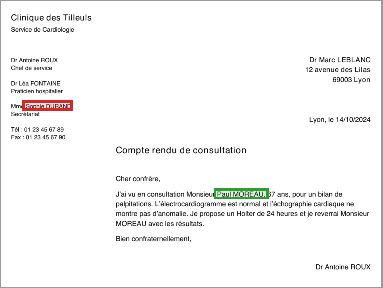
\includegraphics[width=\linewidth]{fig_issue1}\par\smallskip
    \raggedright\footnotesize (a) \textbf{Bandeau du personnel.} «~Mme Sophie DURAND~», la
    secrétaire, vient en premier dans l'ordre de lecture.
    \column{0.48\textwidth}
    \centering
    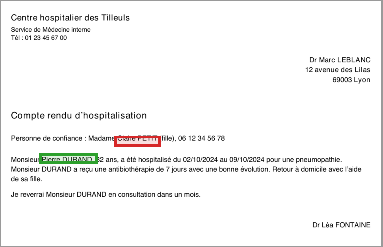
\includegraphics[width=\linewidth]{fig_issue4}\par\smallskip
    \raggedright\footnotesize (b) \textbf{Proche cité en premier.} «~Personne de confiance :
    Madame Claire PETIT~» précède le patient.
  \end{columns}

  \vspace{0.6em}
  \footnotesize \textcolor{tred}{Rouge} : la réponse de la version minimale ;
  \textcolor{tgreen}{vert} : le patient.
\end{frame}

% ---------------------------------------------------------------------------
\begin{frame}{3.2\quad Elle ne trouve rien}
  \begin{columns}[T]
    \column{0.48\textwidth}
    \centering
    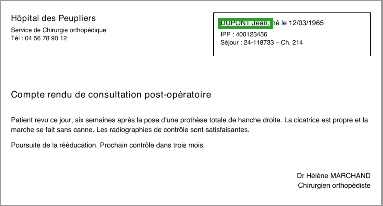
\includegraphics[width=\linewidth]{fig_issue2}\par\smallskip
    \raggedright\footnotesize (a) \textbf{Étiquette d'hôpital.} Le nom n'apparaît que dans
    «~DUPONT Jean, né le 12/03/1965~» : ni civilité, ni \tok{Nom:}.
    \column{0.48\textwidth}
    \centering
    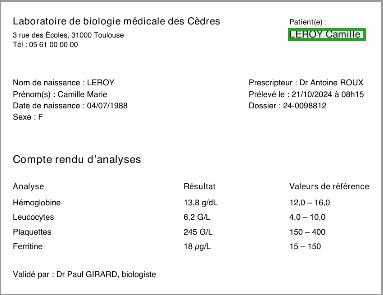
\includegraphics[width=\linewidth]{fig_issue3}\par\smallskip
    \raggedright\footnotesize (b) \textbf{Bloc d'identité.} \tok{Nom de naissance :} et
    \tok{Prénom(s) :} ne sont pas exactement \tok{Nom:} et \tok{Prénom:}.
  \end{columns}

  \vspace{0.6em}
  \footnotesize \textcolor{tgreen}{Vert} : le patient, que la version minimale ne trouve pas
  (elle renvoie \tok{None}).
\end{frame}

% ---------------------------------------------------------------------------
\begin{frame}{3.3\quad Pourquoi elle échoue : trois causes}
  \begin{columns}[T]
    \column{0.30\textwidth}
    \textbf{1. Une seule liste à plat}\par\smallskip
    \small Bandeaux, adresses et signatures sont lus exactement comme la lettre elle-même.
    \column{0.30\textwidth}
    \textbf{2. La première trouvée gagne}\par\smallskip
    \small La première civilité répond, même quand elle désigne une secrétaire ou un proche.
    \column{0.30\textwidth}
    \textbf{3. Deux sortes d'indices}\par\smallskip
    \small Rien pour «~né le~», pour \tok{Nom de naissance :}, ni pour une étiquette placée
    au-dessus du nom.
  \end{columns}

  \vspace{1.6em}
  La correction suit ces trois causes : lire la page \textbf{par blocs}, garder
  \textbf{tous les indices} au lieu du premier, et en reconnaître \textbf{plus de sortes}.
\end{frame}

% ---------------------------------------------------------------------------
\begin{frame}{4\quad La correction : lire la page par blocs, puis voter}
  \begin{columns}[T]
    \column{0.92\textwidth}
    \begin{algo}{\textbf{Algorithme 2 :} version «~mise en page~»}
    \begin{algorithmic}[1]
      \Require un document : des pages, chacune avec ses mots et leurs boîtes
      \Ensure (prénom, nom) du patient, ou \tok{None}
      \State $s(n) \gets 0$ pour tout nom de famille $n$
      \ForEach{page du document}
        \State lignes $\gets$ mots triés par $(y, x)$ ; nouvelle ligne si l'écart en $y$
          dépasse $0{,}005$
        \State morceaux $\gets$ lignes coupées où deux mots sont à plus de $0{,}05$ en $x$
        \State blocs $\gets$ chaque morceau sous le bloc juste au-dessus (même colonne,
          écart $< 0{,}012$)
        \ForEach{bloc dont aucune ligne ne commence par Dr, Pr, Tél ou Fax}
          \ForEach{indice : étiquette (3 points), civilité (2), «~né le~» (2)}
            \State $(p, n) \gets$ au plus deux mots à majuscule après l'indice
              \Comment{capitales : nom}
            \State $s(n) \gets s(n) + \text{points de l'indice}$
          \EndFor
        \EndFor
      \EndFor
      \State $\hat n \gets \arg\max_n s(n)$
      \State \textbf{si} $s(\hat n) \ge 2$, \Return $(\hat p, \hat n)$ ; \textbf{sinon},
        \Return \tok{None}
    \end{algorithmic}
    \end{algo}
  \end{columns}
\end{frame}

% ---------------------------------------------------------------------------
\begin{frame}{4.1\quad Reconstruire la page : lignes, morceaux, blocs}
  \begin{columns}[T]
    \column{0.31\textwidth}
    \centering
    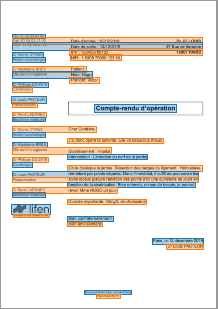
\includegraphics[height=4.5cm]{fig_lines}\par\smallskip
    \raggedright\footnotesize (a) \textbf{40 lignes.} Une nouvelle ligne quand l'écart en $y$
    dépasse $0{,}005$.
    \column{0.31\textwidth}
    \centering
    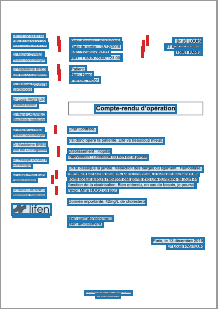
\includegraphics[height=4.5cm]{fig_pieces}\par\smallskip
    \raggedright\footnotesize (b) \textbf{52 morceaux.} Une ligne est coupée (trait rouge)
    quand deux mots sont à plus de $0{,}05$ en $x$.
    \column{0.31\textwidth}
    \centering
    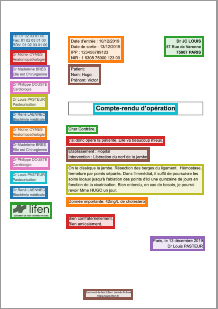
\includegraphics[height=4.5cm]{fig_blocks}\par\smallskip
    \raggedright\footnotesize (c) \textbf{24 blocs.} Un morceau rejoint le bloc juste
    au-dessus, dans la même colonne, si l'écart est $< 0{,}012$.
  \end{columns}

  \vspace{0.5em}
  \footnotesize Document 2, vraies boîtes OCR. Les deux colonnes, mélangées dans les
  lignes (a), sont séparées dans les blocs (c).
\end{frame}

% ---------------------------------------------------------------------------
\begin{frame}{4.2\quad Ignorer les blocs de contact}
  \begin{columns}[T]
    \column{0.52\textwidth}
    \centering
    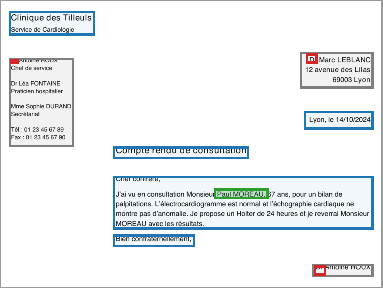
\includegraphics[width=\linewidth]{fig_skip}
    \column{0.44\textwidth}
    \small
    \begin{itemize}
      \item Un bloc dont une ligne commence par un titre de médecin, «~Tél~» ou «~Fax~» est
        ignoré : en-tête, bandeau du personnel, adresse du destinataire, signature.
      \item Ici, «~Mme Sophie DURAND~» est dans le bandeau : elle est ignorée. La seule
        civilité qui reste est «~Monsieur Paul MOREAU~».
    \end{itemize}

    \vspace{0.8em}
    \footnotesize Gris hachuré : bloc ignoré, à cause du mot encadré en
    \textcolor{tred}{rouge} ; \textcolor{tblue}{bleu} : bloc lu ; \textcolor{tgreen}{vert} :
    le patient trouvé.
  \end{columns}
\end{frame}

% ---------------------------------------------------------------------------
\begin{frame}{4.3\quad Trois sortes d'indices, chacune avec des points}
  \begin{center}
    \small
    \renewcommand{\arraystretch}{1.3}
    \begin{tabular}{@{}L{4.6cm}L{6.4cm}c@{}}
      \toprule
      \textbf{Indice} & \textbf{Exemple} & \textbf{Points} \\
      \midrule
      Étiquette en début de ligne : \tok{Nom}, \tok{Prénom(s)}, \tok{Patient}, jusqu'aux
        deux-points
        & \lab{\tok{Nom de naissance :}} \nm{LEROY},
          \lab{\tok{Prénom(s) :}} \nm{Camille} Marie & 3 \\
      Civilité, sauf juste après un titre de médecin
        & \civ{Monsieur} \nm{Pierre DURAND}, 82 ans & 2 \\
      Naissance : les deux mots avant «~né le~»
        & \nm{DUPONT Jean}, \civ{né le} 12/03/1965 & 2 \\
      \bottomrule
    \end{tabular}
  \end{center}

  \vspace{0.6em}
  \small
  \textbf{Lire le nom.} Au plus deux mots qui commencent par une majuscule, arrêt sur une
  virgule. Un mot tout en capitales est le nom de famille, même s'il vient en premier :
  «~DUPONT Jean~» donne \tok{('Jean', 'DUPONT')}.
\end{frame}

% ---------------------------------------------------------------------------
\begin{frame}{4.4\quad Voter : additionner les points par nom de famille}
  \small
  Soit $\mathcal{C}(n)$ l'ensemble des indices qui donnent le nom de famille $n$ (sans tenir
  compte de la casse). Alors
  \[
    s(n) = \sum_{c \,\in\, \mathcal{C}(n)} \mathrm{points}(c), \qquad
    \hat n = \arg\max_n s(n), \qquad
    \text{réponse} =
    \begin{cases}
      (\hat p, \hat n) & \text{si } s(\hat n) \ge 2,\\
      \texttt{None} & \text{sinon.}
    \end{cases}
  \]

  \vspace{0.2em}
  \begin{center}
    \renewcommand{\arraystretch}{1.25}
    \begin{tabular}{@{}L{2.6cm}L{7.2cm}r@{}}
      \toprule
      \textbf{Nom de famille} & \textbf{Indices trouvés, cas du proche cité en premier}
        & \textbf{Score} \\
      \midrule
      \textbf{DURAND} & «~Monsieur Pierre DURAND~», puis «~Monsieur DURAND~» deux fois
        & $2+2+2 = \mathbf{6}$ \\
      PETIT & «~Madame Claire PETIT~» & $2$ \\
      \bottomrule
    \end{tabular}
  \end{center}

  \vspace{0.4em}
  Réponse : \tok{('Pierre', 'DURAND')}. Le seuil 2 règle le compromis : plus haut, le
  système répond moins souvent mais plus sûrement (moins de faux positifs, plus de faux
  négatifs).
\end{frame}

% ---------------------------------------------------------------------------
\begin{frame}{4.5\quad Résultats : les quatre cas sont corrigés}
  \begin{center}
    \small
    \renewcommand{\arraystretch}{1.25}
    \begin{tabular}{@{}L{2.8cm}L{2.4cm}L{2.4cm}L{4.7cm}@{}}
      \toprule
      \textbf{Document} & \textbf{Version minimale} & \textbf{Mise en page} & \textbf{Ce qui corrige} \\
      \midrule
      Bandeau du personnel & \textcolor{tred}{Sophie DURAND} & \textcolor{tgreen}{Paul MOREAU}
        & le bandeau est ignoré : ses lignes commencent par «~Dr~» et «~Tél~» \\
      Étiquette d'hôpital & \tok{None} & \textcolor{tgreen}{Jean DUPONT}
        & l'indice «~né le~», puis les capitales : DUPONT est le nom \\
      Bloc d'identité & \tok{None} & \textcolor{tgreen}{Camille LEROY}
        & les étiquettes \tok{Nom de naissance :} et \tok{Prénom(s) :} \\
      Proche cité en premier & \textcolor{tred}{Claire PETIT} & \textcolor{tgreen}{Pierre DURAND}
        & le vote : DURAND 6 points, PETIT 2 \\
      \bottomrule
    \end{tabular}
  \end{center}

  \vspace{0.6em}
  \small Les trois documents du challenge donnent toujours les mêmes réponses.
\end{frame}

% ---------------------------------------------------------------------------
\begin{frame}{4.6\quad Mesurer : précision, rappel et F1}
  \small
  Pour chaque document : une \textbf{bonne réponse} est un vrai positif (VP) ; un
  \textbf{mauvais nom} est un faux positif (FP) et manque le patient (FN) ; \textbf{aucune
  réponse} est un faux négatif (FN).
  \[
    \text{précision} = \frac{\mathrm{VP}}{\mathrm{VP} + \mathrm{FP}}, \qquad
    \text{rappel} = \frac{\mathrm{VP}}{\mathrm{VP} + \mathrm{FN}}, \qquad
    F_1 = \frac{2 \cdot \text{précision} \cdot \text{rappel}}{\text{précision} + \text{rappel}}
  \]

  \begin{center}
    \renewcommand{\arraystretch}{1.25}
    \setlength{\tabcolsep}{5pt}
    \begin{tabular}{@{}lccccccc@{}}
      \toprule
      & \multicolumn{3}{c}{\textbf{Issue des 7 documents}} & & & \\
      \cmidrule(lr){2-4}
      \textbf{Version} & bonne & mauvais nom & aucune & \textbf{Précision} & \textbf{Rappel}
        & $\mathbf{F_1}$ \\
      \midrule
      Minimale & 3 & 2 & 2 & $3/5 = \pct{60}$ & $3/7 \approx \pct{43}$ & $0{,}50$ \\
      Mise en page & 7 & 0 & 0 & $7/7 = \pct{100}$ & $7/7 = \pct{100}$ & $1{,}00$ \\
      \bottomrule
    \end{tabular}
  \end{center}

  \footnotesize
  Sur les 7 documents de cette présentation (les 3 du challenge et les 4 cas). Ils ont été
  choisis pour montrer les échecs : ce n'est pas une évaluation. Il faut un jeu de test annoté
  plus grand, et faire varier le seuil du vote : c'est la suite.
\end{frame}

% ---------------------------------------------------------------------------
% Les deux courbes lisent figures/roc_minimal.dat et figures/roc_layout.dat, écrits par
% evaluation/roc.py sur le jeu de evaluation/make_test_set.py. Les nombres du texte viennent
% de la sortie de roc.py.
\begin{frame}{4.7\quad Faire varier le seuil : la courbe ROC}
  \begin{columns}[T]
    \column{0.41\textwidth}
    \centering
    \begin{tikzpicture}
      \begin{axis}[courbe,
          xlabel={FPR : fausses acceptées / fausses},
          ylabel={TPR : justes acceptées / justes},
          legend style={at={(0.98,0.03)}, anchor=south east}]
        \addplot[black!45, dashed, forget plot] coordinates {(0,0) (1,1)};
        \addplot[minimale] table[x=fpr, y=tpr] {figures/roc_minimal.dat};
        \addlegendentry{minimale}
        \addplot[miseenpage] table[x=fpr, y=tpr] {figures/roc_layout.dat};
        \addlegendentry{mise en page}
        \addplot[seuilactuel] coordinates {(1,1)};
        \addlegendentry{seuil actuel}
        \node[seuil, anchor=west] at (axis cs:0.025,0.030) {8};
        \node[seuil, anchor=west] at (axis cs:0.045,0.105) {6};
        \node[seuil, anchor=south east] at (axis cs:0.075,0.340) {4};
        \node[seuil, anchor=south east] at (axis cs:0.415,0.605) {3};
        \node[font=\scriptsize, text=black!55, rotate=45] at (axis cs:0.62,0.55) {hasard};
      \end{axis}
    \end{tikzpicture}\par
    {\scriptsize\color{mlgray} Nombres : seuils $\tau$ (mise en page).\par
    \medskip
    Jeu de test : 500 documents synthétiques, 6 sortes (lettres, étiquettes, biologie…), noms
    tirés au hasard. Le mélange est notre choix : les chiffres en dépendent.\par}

    \column{0.55\textwidth}
    \small
    \begin{itemize}\setlength{\itemsep}{1pt}
      \item \textbf{Score $c$.} Mise en page : $c = s(\hat n)$, le total des votes.
        Minimale : $c = 2$ si la règle~1 répond, $1$ pour la règle~2.
      \item \textbf{Seuil $\tau$.} Si $c \ge \tau$, la réponse est acceptée ; sinon,
        vérification humaine. Un seuil donne un point.
      \item \textbf{Positif} : réponse juste, prénom et nom exacts. Les documents sans
        réponse ne sont pas sur la courbe.
      \item \textbf{AUC} $= \Pr(c_{\text{juste}} > c_{\text{fausse}})$, égalité :
        $\tfrac12$. Ici $0{,}61$ et $0{,}63$ ; hasard : $0{,}5$ ; parfait : $1$.
      \item \textbf{Seuil actuel} (orange) : \tok{MIN\_SCORE = 2} accepte tout, car chaque
        indice vaut au moins 2 points.
    \end{itemize}
  \end{columns}
\end{frame}

% ---------------------------------------------------------------------------
\begin{frame}{4.8\quad Précision et rappel selon le seuil}
  \begin{columns}[T]
    \column{0.41\textwidth}
    \centering
    \begin{tikzpicture}
      \begin{axis}[courbe,
          xlabel={Rappel : justes acceptées / documents},
          ylabel={Précision : justes / acceptées}, ymax=1.06,
          legend style={at={(0.03,0.03)}, anchor=south west}]
        \addplot[minimale] table[x=recall, y=precision] {figures/roc_minimal.dat};
        \addlegendentry{minimale}
        \addplot[miseenpage] table[x=recall, y=precision] {figures/roc_layout.dat};
        \addlegendentry{mise en page}
        \addplot[seuilactuel] coordinates {(0.352,0.542) (0.738,0.797)};
        \addlegendentry{seuil actuel}
        \node[seuil, anchor=south west] at (axis cs:0.025,1.0) {8};
        \node[seuil, anchor=north east] at (axis cs:0.075,0.945) {6};
        \node[seuil, anchor=north] at (axis cs:0.244,0.925) {4};
        \node[seuil, anchor=north] at (axis cs:0.44,0.833) {3};
        \node[seuil, anchor=north] at (axis cs:0.738,0.765) {2};
        \node[seuil, anchor=west] at (axis cs:0.10,0.99) {règle 1};
        \node[seuil, anchor=north] at (axis cs:0.352,0.51) {règles 1 et 2};
      \end{axis}
    \end{tikzpicture}\par
    {\scriptsize\color{mlgray} Un point par seuil $\tau$ ; orange : seuil actuel.\par
    \medskip
    Mêmes 500 documents. IC à \pct{95} de l'AUC (bootstrap) : [$0{,}58$ ; $0{,}64$] pour la
    minimale, [$0{,}58$ ; $0{,}68$] pour la mise en page.\par}

    \column{0.55\textwidth}
    \centering
    {\footnotesize
    \renewcommand{\arraystretch}{1.05}
    \begin{tabular}{@{}lcc@{}}
      \toprule
      \textbf{Seuil actuel} & \textbf{Minimale} & \textbf{Mise en page} \\
      \midrule
      bonne réponse & 176 & 369 \\
      mauvais nom & 149 & 94 \\
      aucune réponse & 175 & 37 \\
      \midrule
      Précision & \pct{54} & \pct{80} \\
      Rappel & \pct{35} & \pct{74} \\
      $F_1$ & $0{,}43$ & $0{,}77$ \\
      AUC & $0{,}61$ & $0{,}63$ \\
      \bottomrule
    \end{tabular}\par}

    \medskip
    \raggedright\small
    \begin{itemize}\setlength{\itemsep}{1pt}
      \item AUC proches, mais deux fois plus de bons noms : la ROC ignore les documents
        sans réponse.
      \item Seuil 4 : précision \pct{94}, rappel \pct{24}. À 3 points, 27 mauvais noms sur
        32 sont des fiches à deux colonnes, où \tok{Nom :} lit «~Date~».
    \end{itemize}
  \end{columns}
\end{frame}

% ---------------------------------------------------------------------------
\begin{frame}{5\quad À retenir : les règles marchent, jusqu'à la prochaine mise en page}
  \begin{columns}[T]
    \column{0.30\textwidth}
    \textbf{Version minimale}\par\smallskip
    {\Large 62} lignes\par\smallskip
    \small Deux règles. Juste sur les trois documents du challenge, fausse ou vide sur les
    quatre cas ordinaires.
    \column{0.30\textwidth}
    \textbf{Version mise en page}\par\smallskip
    {\Large 112} lignes\par\smallskip
    \small Blocs, indices et votes. Corrige les quatre cas, mais un formulaire dont les
    valeurs sont loin de leurs étiquettes la met encore en échec.
    \column{0.30\textwidth}
    \textbf{Ensuite : apprendre}\par\smallskip
    {\Large Partie 2}\par\smallskip
    \small Les règles couvrent les cas un par un, et leur score sépare mal le juste du faux
    (AUC $0{,}63$). Un modèle apprend ces régularités à partir de documents annotés.
  \end{columns}

  \vspace{1.4em}
  \footnotesize Lignes de code sans commentaires ni lignes vides.
\end{frame}

\end{document}
